\section*{Exercise 3}





1. Make a figure to describe the architecture of your CNN. Specify the corresponding
hyper-parameters and trainable parameters used in every layer of your network. Cal-
culate manually the output size of each layer. \\
2. What is the total number of trainable parameters of your network? Report the results
you get after certain number of epochs (e.g. 50) and compare them with the results
obtained from VGGNet.\\

For our 4-layer CNN, we chose 3 convolution layers followed by average pooling and a fully connected layer. As an activation function, we used ReLu and we added a dropout layer after the 3rd convolution layer. The figures below show the differences between the same CNN with the dropout layer and without.

\begin{figure}[H]
    \centering
    \begin{subfigure}[t]{0.48\textwidth}
        \centering
        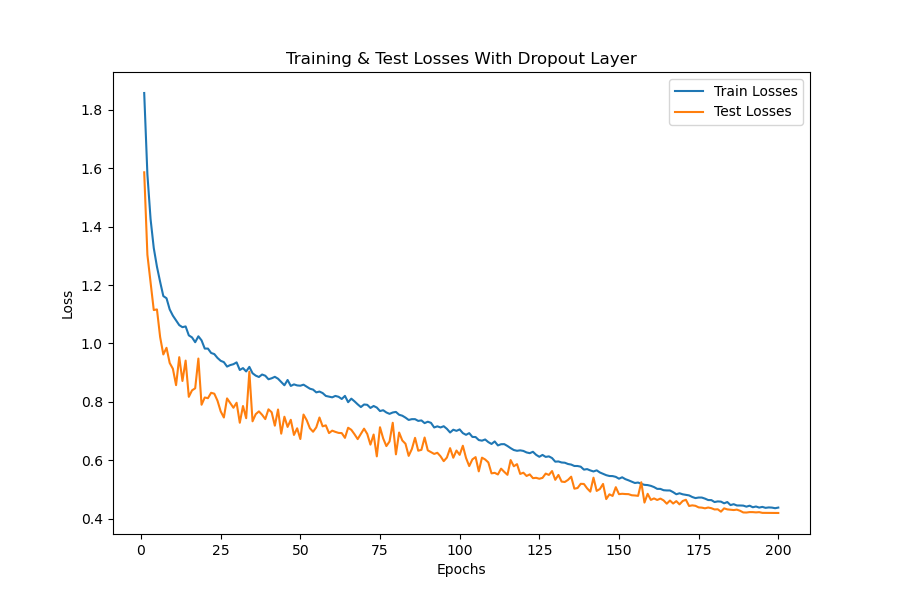
\includegraphics[width=\textwidth]{images/ex_3_Training & Test Losses With Dropout Layer.png}
        \caption{Average training vs. test loss with Dropout Layer.}
    \end{subfigure}
    \hfill
    \begin{subfigure}[t]{0.48\textwidth}
        \centering
        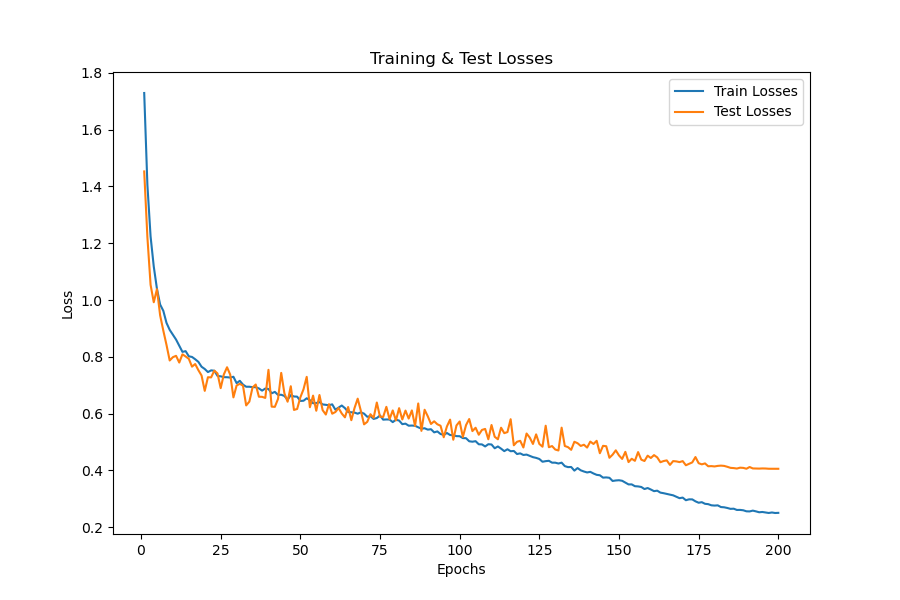
\includegraphics[width=\textwidth]{images/ex_3_Training & Test Losses.png}
        \caption{Average training vs. test loss without Dropout Layer.}
    \end{subfigure}
    \caption{Training vs. Test Loss with/out Dropout}
\end{figure}

\begin{figure}[H]
    \centering
    \begin{subfigure}[t]{0.48\textwidth}
        \centering
        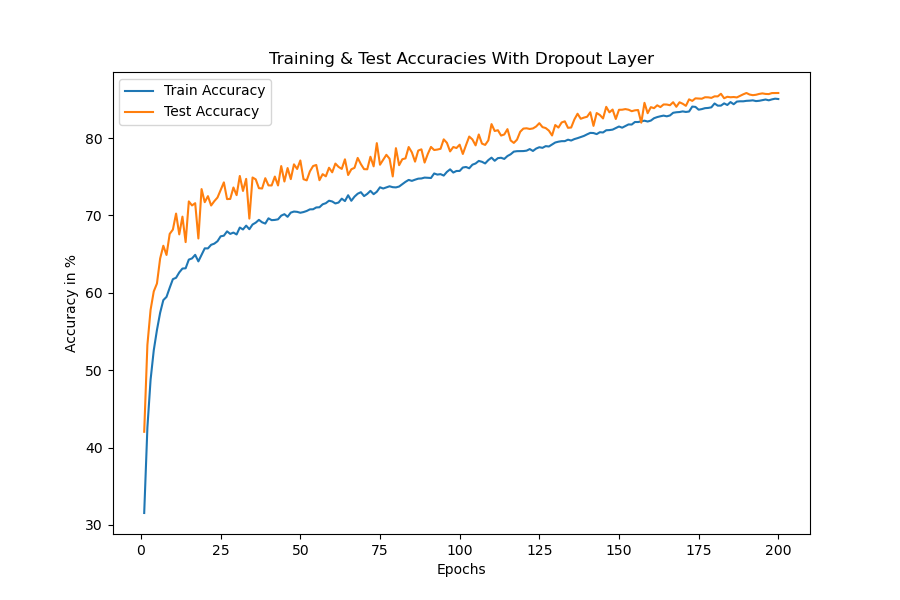
\includegraphics[width=\textwidth]{images/ex_3_Training & Test Accuracies With Dropout Layer.png}
        \caption{Average training vs. test accuracy with Dropout Layer.}
    \end{subfigure}
    \hfill
    \begin{subfigure}[t]{0.48\textwidth}
        \centering
        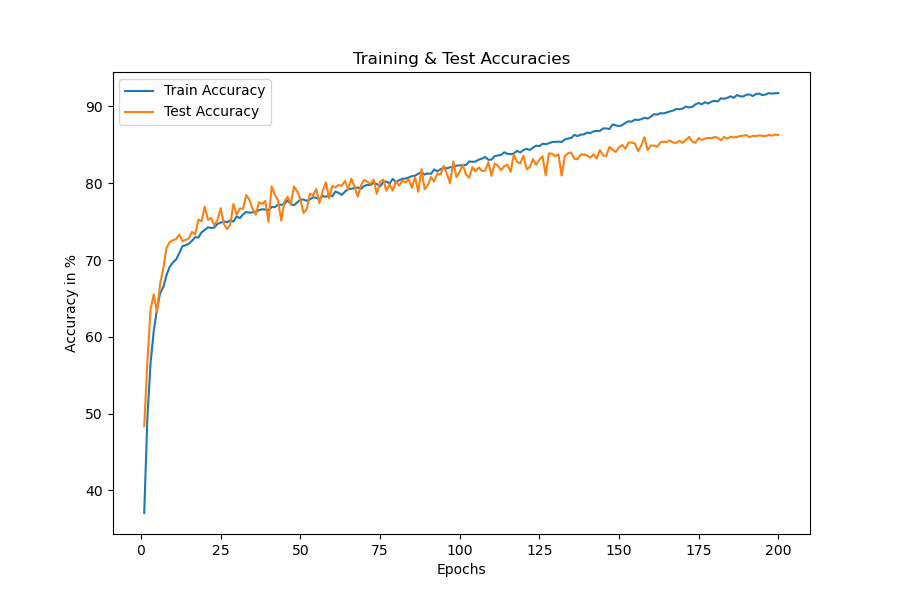
\includegraphics[width=\textwidth]{images/ex_3_Training & Test Accuracies.png}
        \caption{Average training vs. test accuracy without Dropout Layer.}
    \end{subfigure}
    \caption{Training vs. Test Accuracy with/out Dropout}
\end{figure}

\begin{figure}[H]
    \centering
    \begin{subfigure}[t]{0.48\textwidth}
        \centering
        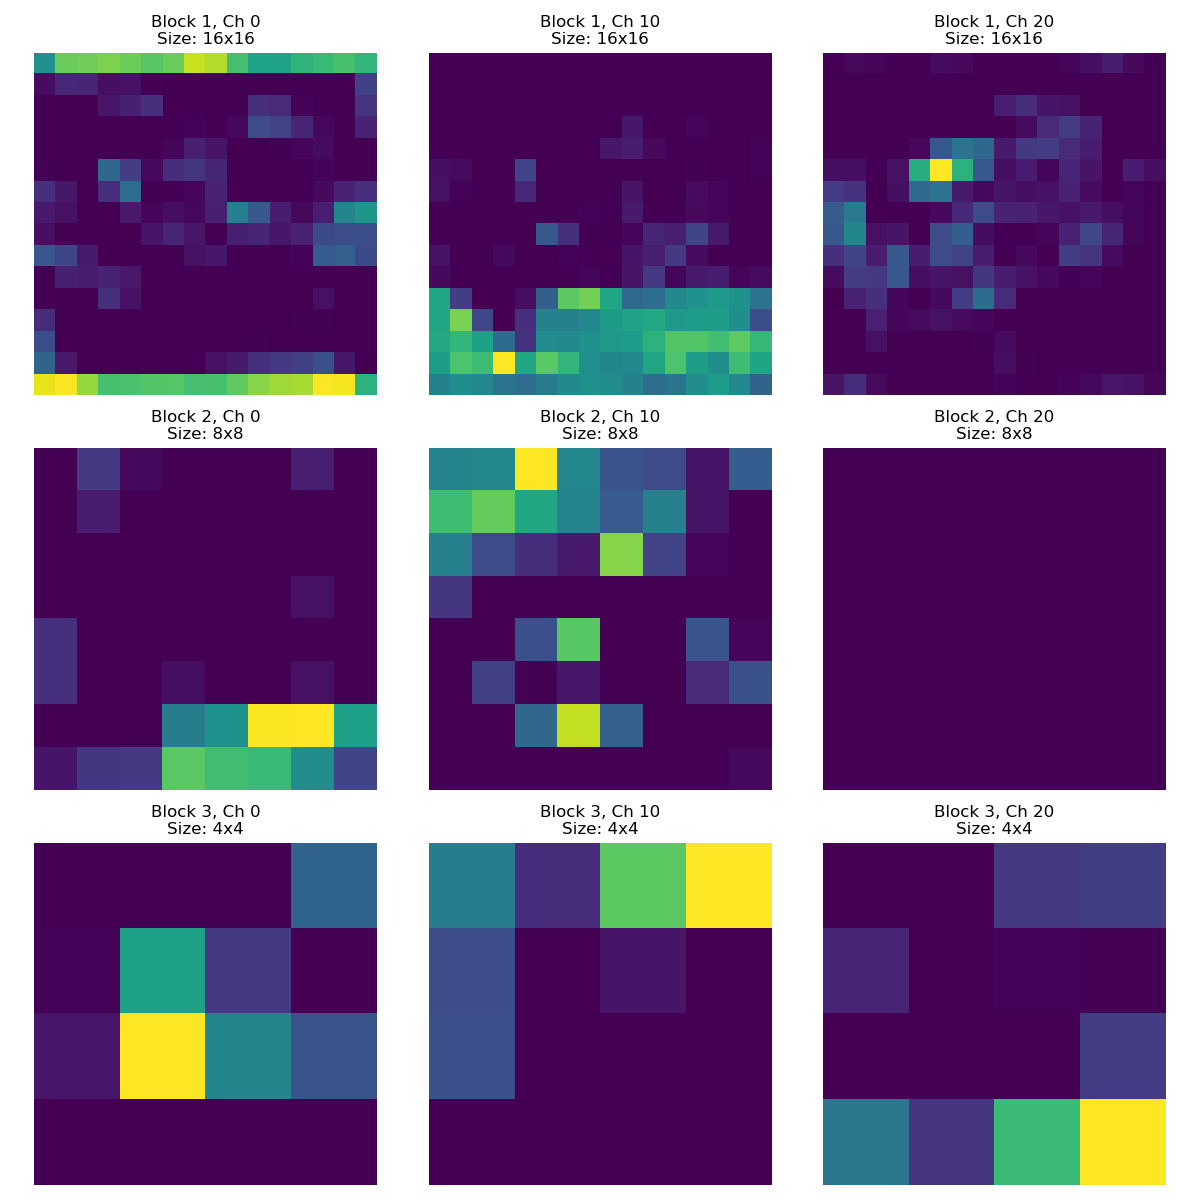
\includegraphics[width=\textwidth]{images/ex_3_feature_maps_visualization_dropout.png}
        \caption{Feature maps across 3 convolutional layers with Dropout Layer.}
    \end{subfigure}
    \hfill
    \begin{subfigure}[t]{0.48\textwidth}
        \centering
        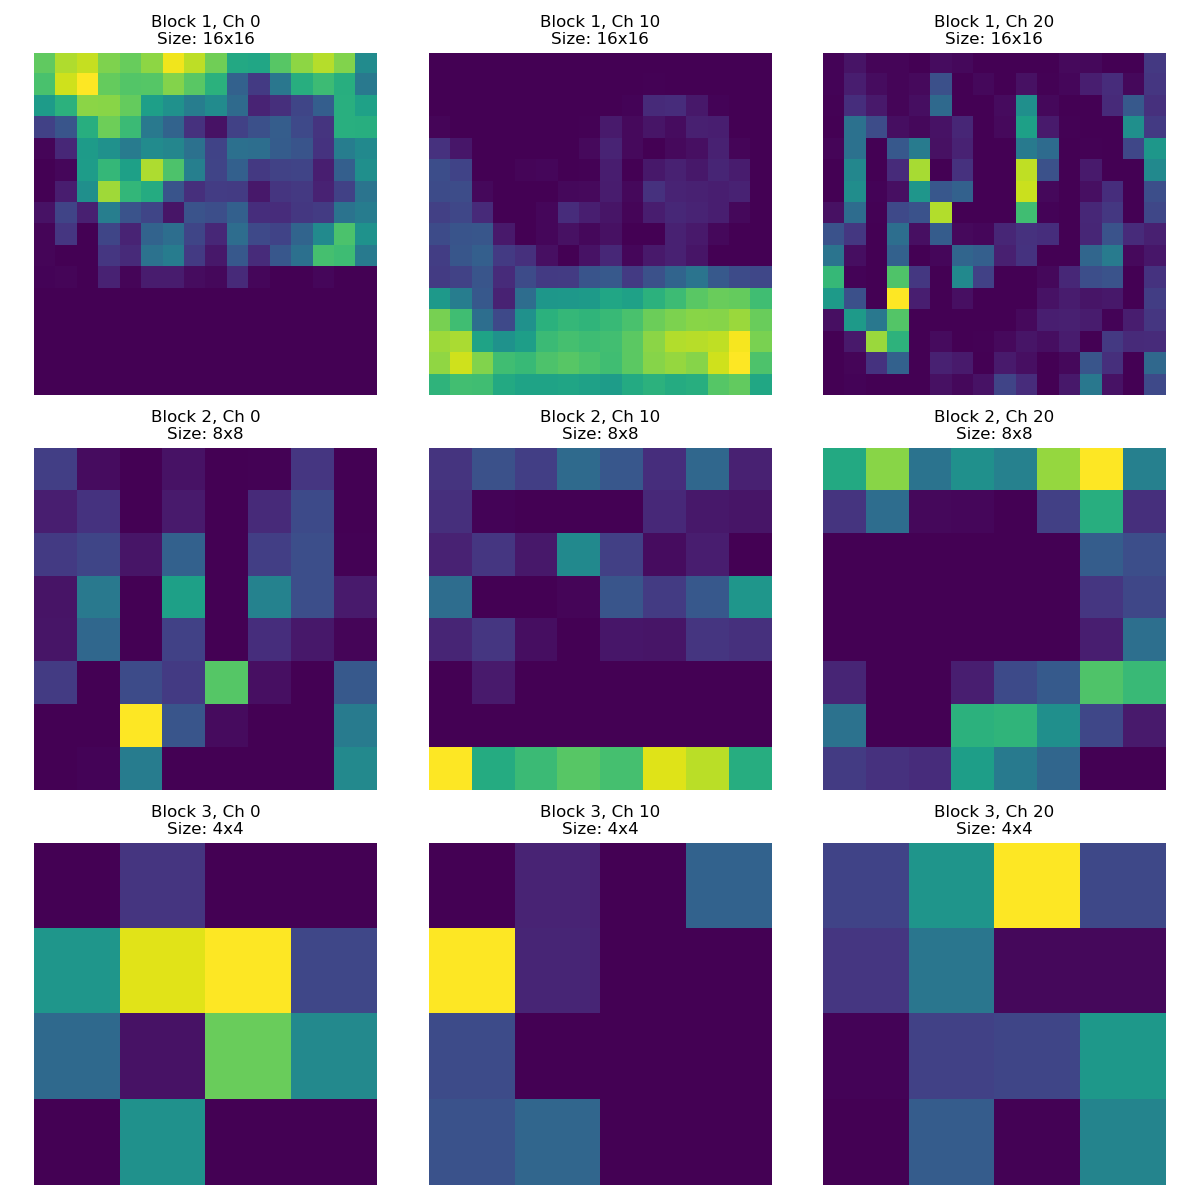
\includegraphics[width=\textwidth]{images/ex_3_feature_maps_visualization.png}
        \caption{Feature maps across 3 convolutional layers without Dropout Layer.}
    \end{subfigure}
    \caption{Feature maps across 3 convolutional layers with/out Dropout Layer.}
\end{figure}

\textbf{Loss}\\
The CNN with the dropout layer shows that the training and test losses are close, reducing overfitting. The CNN model without dropout creates a gap between the training and testing showing a poor generalization of data.

\textbf{Accuracy}\\
The CNN with the dropout layer shows less overfitting as the training and test accuracy curves remain closer throughout the training process, leading to a much smoother increase in test accuracy. The CNN model without dropout shows a clea sign of overfitting after aprox. 100 epochs where training accuracy continues to increase, but test accuracy plateaus significantly lower.

\textbf{Feature Maps}\\
The main difference between the feature maps is that the dropout layer propagates back through the network changing the final weight values of all previous layers.


